\chapter{引言}
\label{cha:intro}

\section{选题背景}

\subsection{云计算的历程}
\label{subsec:history-of-cloud}

云计算的概念诞生的远远比它的名字更早。它的概念可以追溯到早期的
分时系统 (time-sharing systems)。

早期的计算机系统价格昂贵,而且体积庞大,使得个人用户很难拥有独立的个人计算机 (PC) 。
这就导致了多个用户可以同时使用同一个计算资源——例如一台电子计算机——的分时系统
~\cite{timesharing}的产生。所谓分时系统,就是有一个主要的
计算系统 (例如大型机,mainframe computer) ,用户通过终端机 (terminal) 连接到这个
系统上使用计算资源。如图~\ref{fig:unix-time-sharing}所示,威斯康星-麦迪逊分校的学生在
使用终端。用户一般而言不需要考虑计算机操作系统乃至硬件的具体细节——因为自然
有管理员管理这些细节,只需要像“租客”一样使用计算资源就可以了。现代的操作系统,
例如 GNU/Linux 或者 Microsoft Windows ,都支持多用户模式。

\begin{figure}[h]
    \centering
    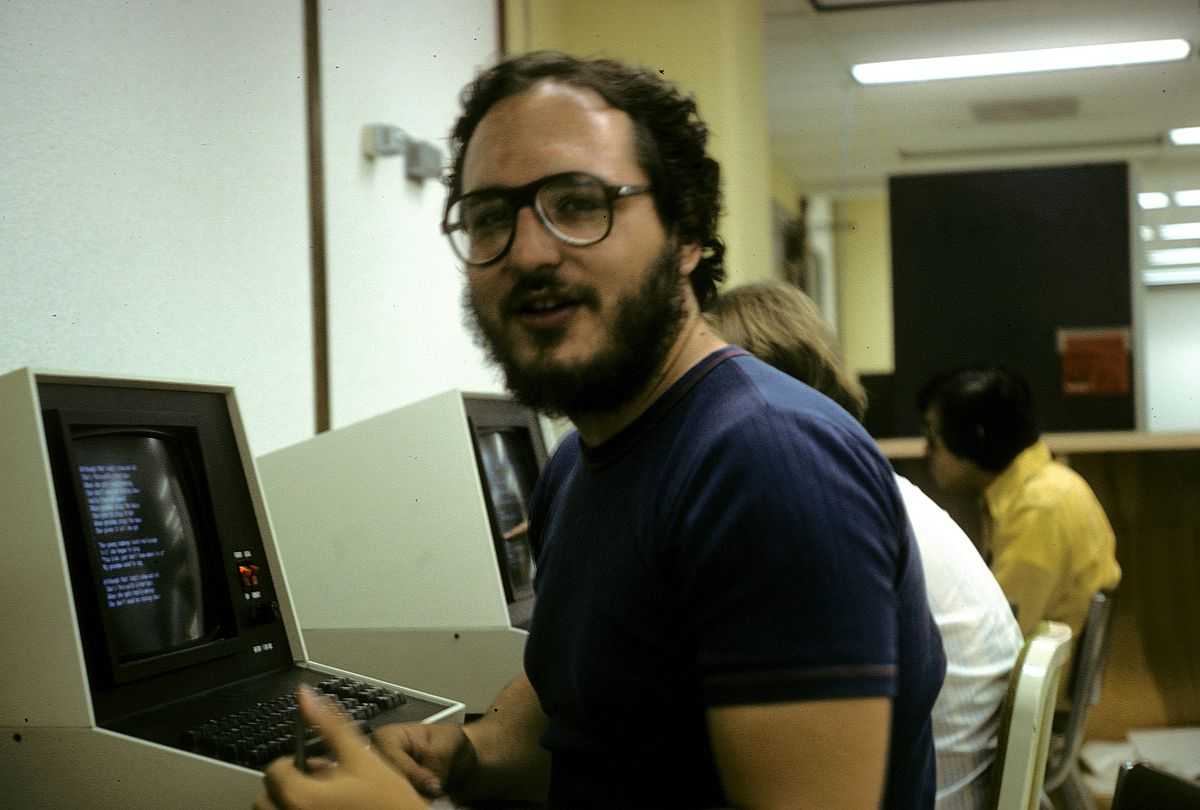
\includegraphics[width=0.7\textwidth]{unix_time_sharing}
    \caption{威斯康辛大学麦迪逊分校的学生使用终端机,1978 年}
    \label{fig:unix-time-sharing}
\end{figure}

从 2000 年左右开始,云计算的概念正式形成了。2006 年诞生的 Amazon EC2 \footnote{EC2
  是 Elastic Compute Cloud 的缩写,因有两个连着的 C 所以叫做 EC2 ,不是
  “第二个版本”的意思。}成为了迄今最成功的云计算平台之一。2008 年诞生的 OpenNebula
是另一个云计算平台,顾名思义它是一个自由软件\footnote{Free as in freedom}
,使用 Apache License 发布。

而现在更加流行的自由的云计算平台是 OpenStack 。OpenStack 最初是由
 NASA 和 RackSpace 共同发起的,从 2012 年开始由叫做 OpenStack Foundation 的非营利
组织进行开发和维护。它和 Amazon EC2 的最大不同就是它是完全自由和开源的。不但可以利用
这个软件搭建自己的云计算环境,而且可以对相关的代码展开研究。OpenStack 中的主要组成部分
和 Amazon AWS 中的部分具有一定的对应关系,比如 AWS 的核心也就是 EC2 对应了 OpenStack
 里的 Nova ,负责虚拟机的调度和管理;AWS 中的简单存储模块 S3 在 OpenStack 中
有 Swift 与之对应~\cite{openstack}。

\subsection{云计算平台的服务类型}

\begin{figure}[h]
    \centering
    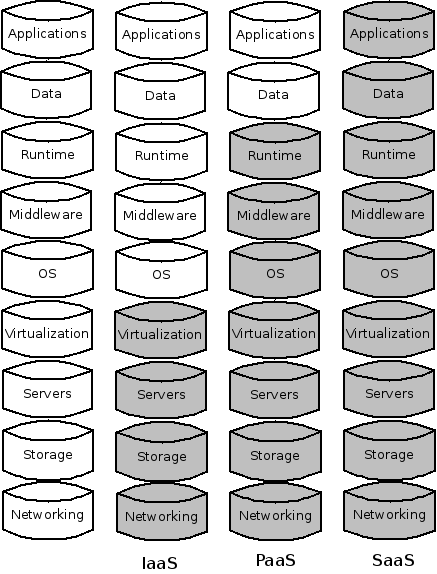
\includegraphics[height=0.4\textheight]{iaas-paas-saas}
    \caption{三种服务类型,灰色部分是由平台提供商管理的部分}
    \label{fig:iaas-paas-saas}
\end{figure}

云计算提倡的概念是“所有都是服务”
 (everything as a service) ~\cite{cloud-and-openstack},也就是用户不直接接触
物理上的计算机,但是却能通过网络获得相应的计算服务。云计算的“云”不在本地,这就好比大家
每天日常生活都要使用电,但极少有人在家里自己搭建一台柴油发电机,而是在发电厂集中发电,
然后通过输电线路把电力输送到千家万户供人们使用。数据中心就好像这个发电厂,计算机网络
就好像电线,终端用户就像使用电力一样使用云计算产生的计算资源。

根据服务类型不同,云计算平台主要可以分为以下三种——基础设施
服务 (IaaS)、平台服务 (PaaS) 还有软件服务 (SaaS) ~\cite{types-of-cloud},
它们的区别是服务提供商提供的解决方案包含的部分占整个软件栈的比例,如图
~\ref{fig:iaas-paas-saas}所示。

\subsubsection{基础设施服务}
\label{subsubsec:iaas}

顾名思义,这种服务类型就是只提供必要的设施,而不提供上层应用。这些设施包括由虚拟机管理程序
 (hypervisor) 支持的大量的虚拟机集群、操作系统磁盘镜像存储池(这样用户在创建虚拟机实例的
时候就不用联网从镜像源下载镜像,直接从镜像存储服务调取相应的镜像即可)、文件存储服务、
防火墙、负载均衡器等等。

当然还有虚拟局域网 (VLAN)。例如某大学计算机系有网络和操作系统两个实验室,它们共享一套虚拟
机集群。网络实验室和操作系统实验室希望各占用一个子网。如果是使用物理上的局域网,那么应该有
两个交换机,各接入路由器的两个物理端口上。而使用了虚拟局域网,就可以用两个逻辑端口代替。
使用虚拟局域网,可以缩小广播域,从而提高集群的安全性。

\begin{figure}[h]
    \centering
    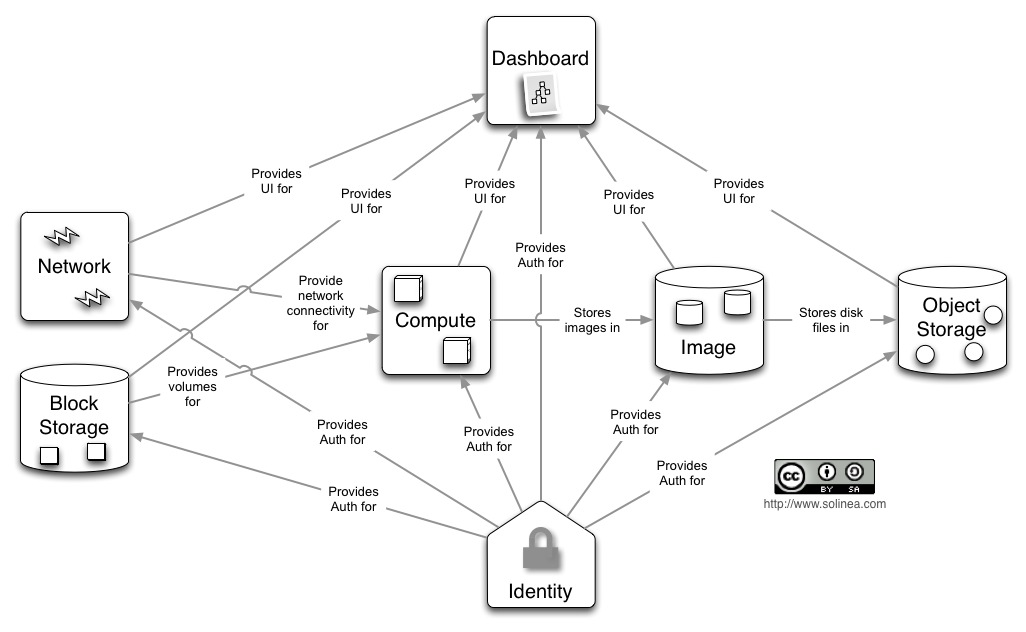
\includegraphics[width=\textwidth]{openstack-conceptual-diagram}
    \caption{OpenStack 的概念架构图(来自 OpenStack 官方电子手册)}
    \label{fig:openstack-conceptual-diagram}
\end{figure}

上文提到的 Amazon EC2 就是一个典型的 IaaS 平台。类似的,OpenStack 也是一个 IaaS 平台,
如图~\ref{fig:openstack-conceptual-diagram}。截至到 2016 年,一共包含以下几个核心
组成部分~\cite{openstack}:

\begin{enumerate}
    \item \textbf{Nova:} Nova 是 OpenStack 的计算部分,主要负责虚拟机管理。它的 API
    可以和 Amazon EC2 的相兼容,RackSpace 和惠普~\cite{hpe-openstack}的商业计算服务
    就是建立在 Nova 上的,Nova 的基本架构如图~\ref{fig:openstack-nova-arch}所示。
    Nova 主要包含以下几个组件\footnote{实际上还有 nova-cert 和 nova-objectstore ,
    但不是主要的}:
    \begin{figure}[h]
        \centering
        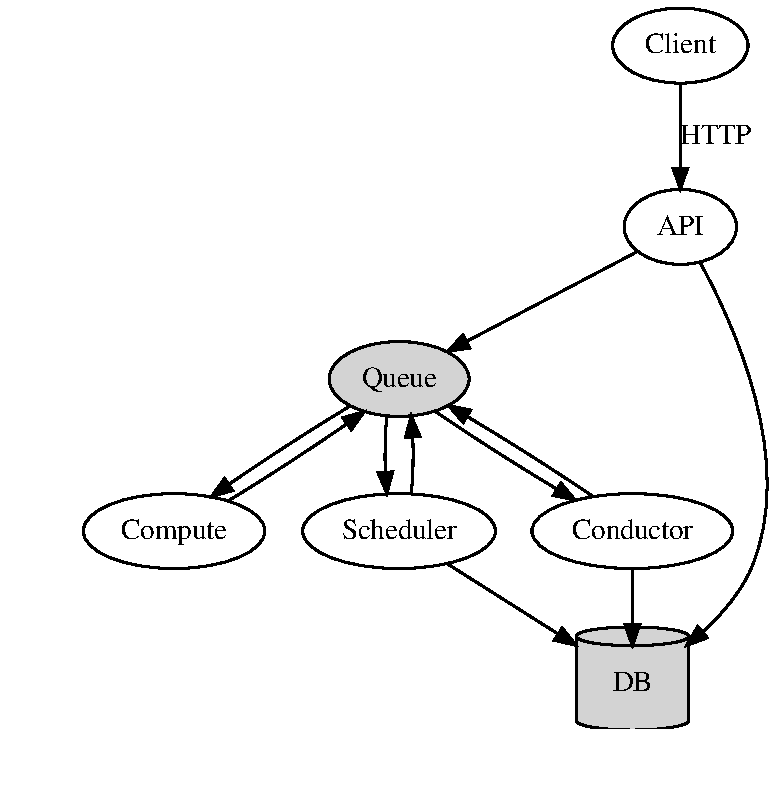
\includegraphics[width=0.7\textwidth]{openstack-nova-arch}
        \caption{OpenStack Nova 的架构图}
        \label{fig:openstack-nova-arch}
    \end{figure}
    \begin{enumerate}
        \item \textbf{nova-compute:} 这是 Nova 用来管理虚拟机的模块。它安装在物理集群
        中的每台机器上,主要负责接收用户对虚拟机的操作,例如创建删除等。这些操作依赖底层的
        虚拟机管理程序 (hypervisor) 提供的 API ,如 XenAPI 、VMWareAPI
         或者 libvirt 。
        \item \textbf{nova-scheduler:} 是一个调度器,负责协调例如在哪台物理机上创建
        新的虚拟机这样的调度工作。可以灵活的通过配置文件配置。
        \item \textbf{nova-conductor:} 负责安全的组件。nova-compute 进行的数据库
        操作,需要由 nova-conductor 代为转交给 nova-db 进行处理。它设计的目的是为了
        防止 nova-compute 直接访问数据库,所以不能和 nova-compute 一样直接部署在
        物理计算节点上,不然就失去了保障安全的效果了。~\cite{conductor}
        \item \textbf{nova-db:} 数据库,记录租户信息、虚拟机状态、物理机状态等。实际上
        因为 nova 是使用 Python 实现的,所以数据库接口部分使用的是 SQLAlchemy
         \footnote{\url{http://www.sqlalchemy.org/}},可以使用任何 SQLAlchemy
         兼容的数据库。
        \item \textbf{nova-console:} 顾名思义,Nova 的控制台服务。
    \end{enumerate}
    \item \textbf{Neutron:} OpenStack 的虚拟网络服务叫做 Neutron ,它的前身是
     nova-network 。它的理念是“网络作为服务”\footnote{Network as a service}。
    它允许用户创建虚拟网络并连接网络设备的接口。Neutron 有一个主要的服务进程
     neutron-server 运行在网络控制节点上,它接受用户发来的 HTTP 请求,发送给遍布
    物理集群的机器上运行的 agent 进行处理。为了更容易扩展,Neutron 提供 plugin 机制,
    每个 plugin 提供一组特定的 API ,通过 RPC 调用 agent 完成操作。
    \begin{figure}[h]
        \centering
        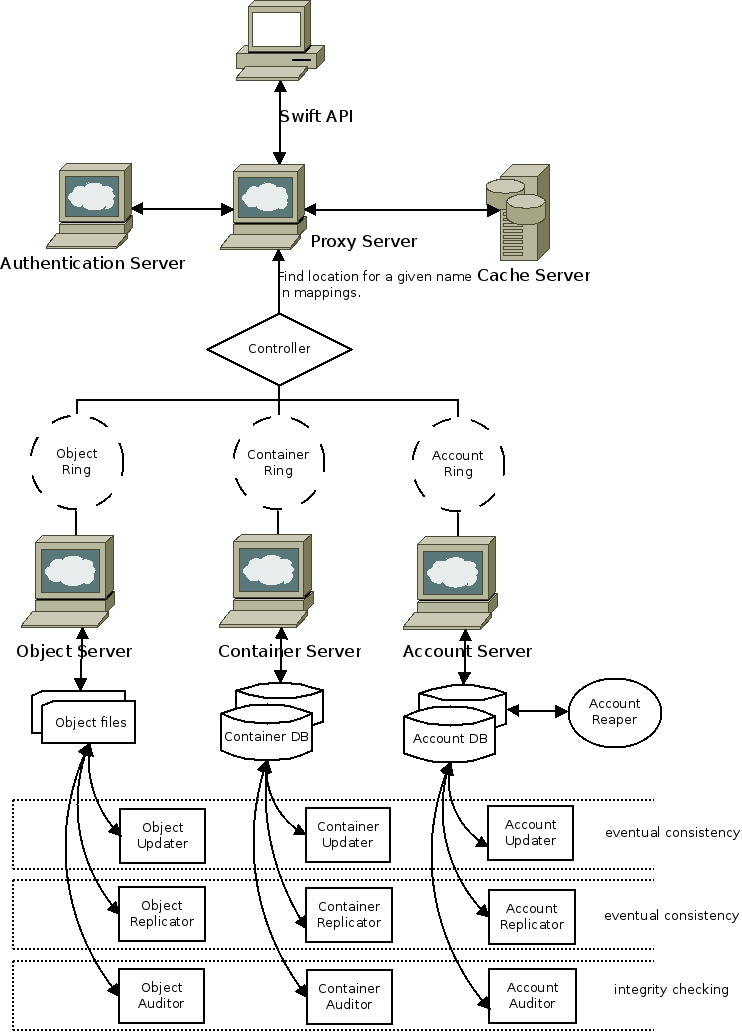
\includegraphics[height=0.7\textheight]{openstack-swift-arch}
        \caption{OpenStack Swift 的架构图}
        \label{fig:openstack-swift-arch}
    \end{figure}
    \item \textbf{Swift:} Swift 项目是 OpenStack 提供的对象存储 (Object Storage)
     服务\footnote{对于程序员来说,这个概念容易和“面向对象”中的对象相混淆,前者是指在
    云端存储的一个文件,后者是对具有一定行为特征的一类概念的抽象},其基本结构如图
    ~\ref{fig:openstack-swift-arch}所示。一个 IaaS 服务框架,
    为什么要提供存储服务呢?物理世界中,一般使用存储区域网络
     (SAN) 或者网络附属存储 (NAS) 来保证数据的集中管理。在虚拟化的世界中,虚拟机数据的
    集中存储更是至关重要,因为虚拟机的临时存储好比无源之水、无本之木,随着虚拟机的删除,
    它存储的数据也就消失了。对象存储和快存储就是为了解决这个问题,好把数据统一管理起来。
    OpenStack 里的对象存储就是 Swift ,Swift 又分为访问层和存储层两部分,分别负责
    RESTful 请求的处理、权限控制和实际对象数据的存储。Swift 主要应用在不容易发生变化的
    数据文件上,例如磁盘镜像文件和备份文件,当然还有大的媒体文件。
    \begin{figure}[h]
        \centering
        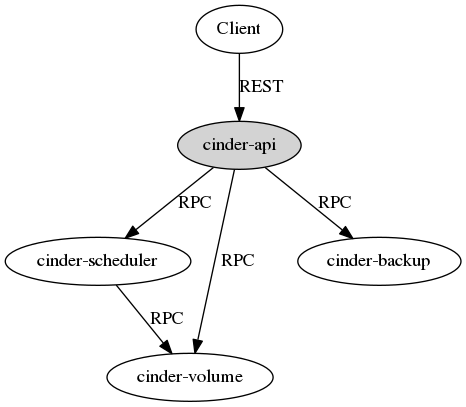
\includegraphics[width=0.7\textwidth]{openstack-cinder-arch}
        \caption{OpenStack Cinder 的架构图}
        \label{fig:openstack-cinder-arch}
    \end{figure}
    \item \textbf{Cinder:} Cinder 项目是 OpenStack 提供的块存储 (Block Storage)
     机制,类似于 Amazon EBS (Elastic Block Storage) ,其基本结构如图
    ~\ref{fig:openstack-cinder-arch}。Cinder 提供了逻辑
    存储卷 (volume)的抽象,举例来说,如果数据库服务在一个由 Nova 提供的虚拟机里运行,
    那么一旦虚拟机出错,存储在 Cinder 提供的逻辑存储卷里的数据库还能通过附加 (attach)
     到新的虚拟机上来很快恢复服务,不至于出现“鸡飞蛋打”的情况。从这个意义上,一个 volume
     好比一块移动硬盘,可以在虚拟机之间插拔 (attach 和 detach) 。~\cite{cinder}
    \item \textbf{Glance:} Glance 是 OpenStack 存储三驾马车的最后一架,它是一个镜像
    管理项目,但是本身不负责存储,存储需要依赖 Swift 等项目来实现。它的 API 主要提供了
    镜像 (image) 的导入导出、镜像元数据 (metadata) 的管理等。
    镜像主要有 queued 、saving 、 active 、 killed 、
     deleted 、 pending\_delete 这六个状态。
    \item \textbf{Keystone:} OpenStack 的身份管理系统。
\end{enumerate}

OpenStack 作为 IaaS 开源界的新秀,现在还在不断地发展、完善。

\subsubsection{平台服务}

平台即服务 (PaaS) 是一种给开发者提供的应用程序的开发环境和运行环境
,使得开发者能从繁琐的 IT 环境管理中解放出来~\cite{cloud-and-openstack}。

Google App Engine 就是平台即服务的典型代表。开发者通过使用 Google 提供的
开发套件 (SDK) ,就可以通过云获得 NoSQL 数据存储、内存缓存 (memcache) 、
用户认证等不同服务的 API ,从而搭建出自己的应用程序 (App) 。可以看出,平台
即服务面向的是开发者,提供的是软件的部署和运行的自动化,使开发者能专注于软件
本身的功能。

\subsubsection{软件服务}

\begin{figure}[h]
    \centering
    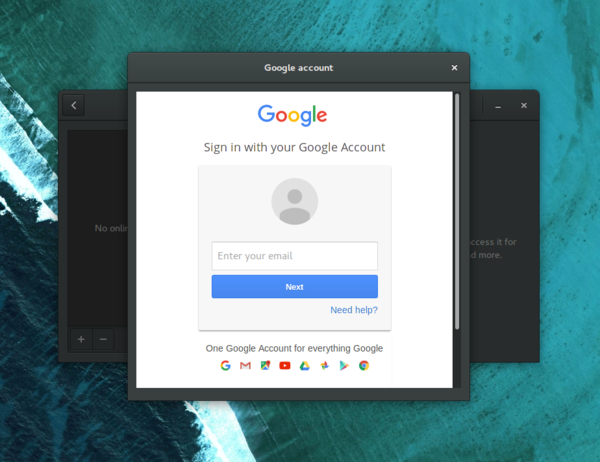
\includegraphics[width=0.7\textwidth]{gnome-google-account}
    \caption{在 Ubuntu 16.04 上的 GNOME 3.18 桌面环境登录 Google 账户}
    \label{fig:gnome-google-account}
\end{figure}

和以上两种形式不同,软件即服务 (SaaS) 既不是面向系统建构师,也不是面向应用开发者,它是
一种面向终端用户的服务形式。用户只要通过浏览器就可以使用相应的软件,而除此之外的工作,
例如软件的部署或是升级,都是由服务提供商在线完成的。

Google Apps 是软件即服务的代表之一。Google 的网页应用程序有邮箱应用 Gmail
 \footnote{\url{https://mail.google.com}}、日历应用 Google Calendar
 \footnote{\url{https://calendar.google.com}}、聊天软件 Google Talk
 \footnote{\url{https://hangouts.google.com}}(现在改名叫 Hangouts )等,
同时它们还提供 API ,使得 Google 的普通应用程序,例如 Android Gapps ,也能和
云端的网页版应用访问相同的数据。第三方开发者也可以八仙过海,各显神通,例如新版的
 GNOME Desktop 就支持 Google 的日历、网盘同步等功能,如图
 ~\ref{fig:gnome-google-account}所示。

\subsection{虚拟化和云计算}

之前在~\ref{subsec:history-of-cloud}节提到了时分复用,从而使不同用户可以利用同一台
计算设备的计算能力,而虚拟化技术就是对硬件设备做的一次抽象,提高了这种复用的效率。

抽象在计算机领域是重要的思维方式,例如 GNU/Linux 的 LVM 技术,就把物理上的磁盘设备
(比如 /dev/sd* )抽象成了逻辑分卷,从而使内核和逻辑分卷而不是物理设备打交道。这样
一个直观的好处就是易于扩展。增加一块磁盘设备,只需要调整逻辑分卷的大小就可以了,在
同一块磁盘上调整不同的分卷也非常方便。另一个好处是扩展了单块磁盘的容量——虽然 RAID 0
也可以达到同样的效果,但是安全性欠佳\footnote{安全性指的是 fault tolerance 和
 redundency,RAID 0 阵列中一盘磁盘失效会导致整个阵列失效},所以 LVM 是更好的实现方法。

虚拟化则是对 CPU 、内存、I/O 、网络等的抽象。通过虚拟机管理程序的模拟,客户虚拟机
(guest) 以为自己是在独占的硬件资源上运行,表现出和物理机相同或者非常类似的行为。而
客户虚拟机之间的资源是互相隔离的,它们运行的操作系统甚至都可以是完全不同的。

把物理计算资源虚拟化成多台逻辑上的计算机,而且它们之间能相互连通,这对于云计算是非常
重要的。现代的计算机单个的性能非常强劲,而有些服务并不需要太多的计算资源,比如搭建
HTTP 服务器提供一个静态的网页,而网页的访问量也不大,那完全没有必要用一“整”台服务器
跑这个服务,而是可以在这个服务器上部署一个虚拟机管理程序,开一个虚拟机来完成这个任务,
余下的计算资源可以分配给其它虚拟机,比如划分一个虚拟机来跑数据库服务。如果以后服务发生了
变化,比如购置了新的服务器,那么可以把其中一些虚拟机快速方便地迁移到新购置的服务器上去。

虚拟化是云计算的基石,虚拟化使得云服务可以方便灵活地伸缩扩展。

\section{研究价值和主要贡献}

通过分析已有的虚拟机(主要是 qemu-kvm )管理程序 NOVA \footnote{NOVA 是清华大学
高性能所学长搭建的一个虚拟机管理平台,而不是 OpenStack Nova }的结构和代码,熟悉
IaaS 平台的开发和编写,还有虚拟集群主机的维护,改写 NOVA 平台支持虚拟容器 LXC 运行
的虚拟环境,实现了 LXC 虚拟容器的自动部署,尝试实现了 LXC 虚拟容器的动态实时迁移。
另外,开发编写了一套基于 Python 和 bash 的适用于虚拟集群的性能测试自动化工具,
测试了常见的负载,包括 HTTP 服务器、memcache 服务、key-value 存储等,
通过性能报告分析了普通虚拟机和虚拟容器的性能差异,并分析了两者资源隔离情况的异同,
为集群虚拟化方案的选型提出了参考意见。

本文的 \LaTeX 源码、全部测试数据图表、NOVA 系统的代码和文档、性能测试工具 Omegabench
的代码和文档都在 GitHub 仓库进行了开源,可以通过互联网自由访问和使用。

\section{论文结构}

本论文的第一章里,简单介绍了云计算的历程和现状,介绍了按照服务类型的分类和各种云计算服务的
特点,概括了云计算和虚拟化的关系。

在第二章,介绍传统虚拟化技术和新型的虚拟容器技术的异同,比较几种虚拟化技术实现上的差异。

在第三章,介绍工作的第一部分,也就是 LXC 虚拟容器分布式管理系统的实现和对 Tsinghua NOVA
已有工作的整合。

在第四章,介绍工作的第二部分,即集群基准测试套件 Omegabench 。并使用该基准测试评估、比较
不同虚拟化方案的性能表现。另外,还通过分析系统的日志,评估 Tsinghua NOVA 系统进行客户机
在宿主机之间迁移的开销。

在第五章,也就是本文的最后一章,总结了全部工作,对虚拟集群虚拟化方案的选型提供了参考意见,
并介绍了项目可能的扩展和改进。
